\documentclass[12pt]{article}

%===============================
%
%          📦 Paquetes
%
%===============================

\usepackage[a4paper, top=2cm, bottom=2cm, left=2.5cm, right=2.5cm]{geometry}
\usepackage[spanish]{babel}
\usepackage[utf8]{inputenc}
\usepackage{amsmath}
\usepackage{multicol}
\usepackage{graphicx}
\usepackage{hyperref}
\usepackage{booktabs}
\usepackage{pgfplots}
\pgfplotsset{compat=1.18}

\title{
  \vspace{2cm}
  \pagenumbering{gobble}
  
\includegraphics[width=5cm]{../assets/logo-utp.png} \\
  \vspace{1cm}
  \textbf{Universidad Tecnológica del Perú} \\
  \vspace{2cm}
  \textbf{Investigación Operativa} \\
  \vspace{1cm}
  \large \textbf{S12 - Evaluación}
}
\author{
  \textbf{Torres Vara, Mateo Nicolas} - \texttt{U24308542} \\
  \texttt{Sección 36373}
}



\begin{document}
\maketitle
\begin{center}

  Docente: Alberto Andre Reyna Alcantara

\end{center}

%======================================
%
%          📚 Inicio del documento
%
%======================================

\newpage
\section*{Ejercicio 1}

\noindent Se tienen 2 plantas que envían producto a 2 centros de distribución, 
los cuales a su vez abastecen a 3 ciudades.
Siendo los datos los siguientes:

\begin{center}
  \begin{tabular}{|c|c|c|c|c|c|}
    \hline
    & CD1 & CD2 & CD3 & CD4 & CD5 \\
    \hline
    Planta A & 3 & 4.5 & 2000 & 15 &  \\
    \hline
    Planta B & 2.8 & 6 & 3000 & 18 &  \\
    \hline
  \end{tabular}
\end{center}

\begin{center}
  \begin{tabular}{|c|c|c|c|c|}
    \hline
    & Ciudad F & Ciudad G & Ciudad H & Capacidad \\
    \hline
    CD1 & 3.5 & 2.5 & 3 & 2800 \\
    \hline
    CD2 & 2 & 4.2 & 3.8 & 1700 \\
    \hline
    Demanda Max & 1500 & 2000 & 2400 & \\
    \hline
    Precio Venta & 45 & 50 & 57 &  \\
    \hline 
  \end{tabular}
\end{center}


\textbf{A. Elabore el modelo correspondiente para maximizar los resultados.}

\vspace{2cm}

\subsection*{Modelo}

\begin{center}
  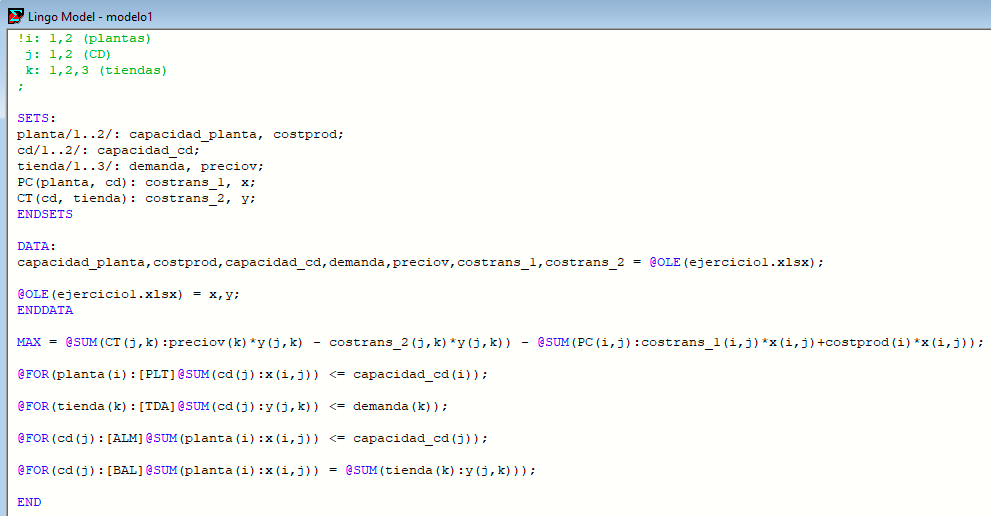
\includegraphics[width=0.8\textwidth]{./assets/model1.PNG}
\end{center}

\subsection*{Modelo Resuelto}
\begin{center}
  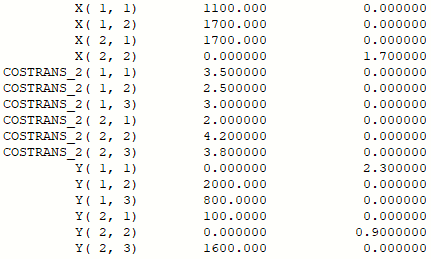
\includegraphics[width=0.8\textwidth]{./assets/solved_model1.PNG}
\end{center}

\subsection*{Tablas de Excel}
\begin{center}
  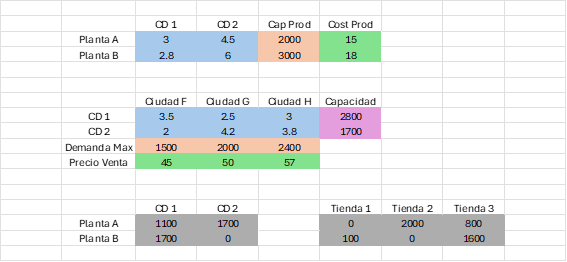
\includegraphics[width=0.8\textwidth]{./assets/excel1.png}
\end{center}






\newpage
\section*{Ejercicio 2}
\noindent La siguiente matriz contiene los costos (en dólares) correspondientes a la asignación de los trabajos 
A, B, C, D y E a las máquinas 1, 2, 3, 4 y 5. Asigne los puestos a las máquinas de modo que los costos se reduzcan al mínimo.
\begin{center}
\begin{tabular}{|c|c|c|c|c|c|}
  \hline
  & \multicolumn{5}{c|}{\textbf{Máquinas}} \\
  \hline
  \textbf{Trabajo} & \textbf{1} & \textbf{2} & \textbf{3} & \textbf{4} & \textbf{5} \\
  \hline
  \textbf{A} & 7 & 10 & 12 & 5 & 11 \\
  \hline
  \textbf{B} & 6 & 11 & 4 & 5 & 9 \\
  \hline
  \textbf{C} & 7 & 14 & 13 & 8 & 10 \\
  \hline
  \textbf{D} & 4 & 10 & 11 & 18 & 13 \\
  \hline
  \textbf{E} & 10 & 5 & 14 & 16 & 12 \\
  \hline
\end{tabular}
\end{center}

\noindent Se pide, \underline{\textbf{dándonos soporte con LINGO}:}
\begin{itemize}
  \item [A.] \textbf{Indique la asignación de cada trabajo a cada máquina.}
  \item [B.] \textbf{Indicar cuál es el costo óptimo de dicha asignación.}
\end{itemize}

\subsection*{Modelo}
\begin{center}
  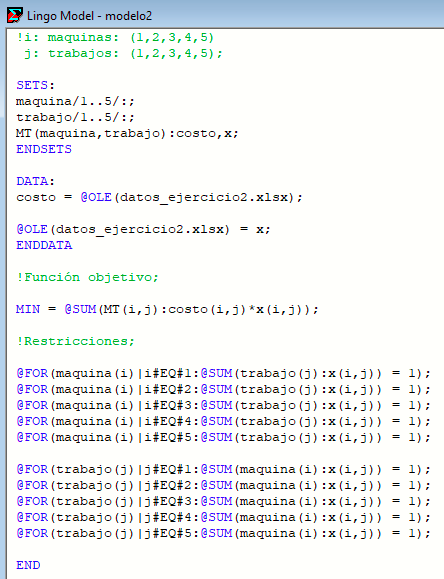
\includegraphics[width=0.7\textwidth]{./assets/model2.PNG}
\end{center}

\subsection*{Modelo Resuelto}
\begin{center}
  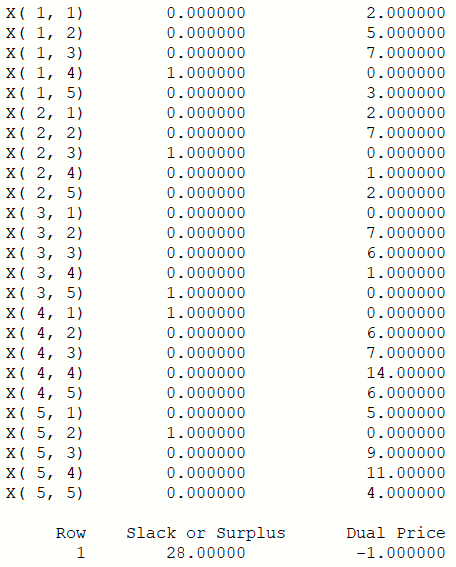
\includegraphics[width=0.5\textwidth]{./assets/solved_model2.PNG}
\end{center}

\subsection*{Tablas de Excel}
\begin{center}
  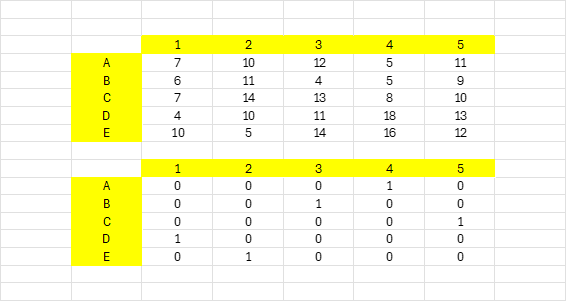
\includegraphics[width=0.8\textwidth]{./assets/excel2.png}
\end{center}

\subsection*{Conclusiones}
\begin{itemize}
  \item [A.] La asignación de trabajos a cada maquina se puede observar en la segunda tabla de excel.
  \item [B.] El costo óptimo de dicha asignación es de 28 dólares.
\end{itemize}

\newpage
\section*{Recursos y créditos}

\begin{itemize}
    \item \textbf{Código fuente:} \href{https://github.com/MateoTVara/UTP/blob/main/docs/C8/Investigacion_Operativa/S12-Evaluacion/evaluacion.pdf}{Repositorio GitHub - Investigación Operativa}
    \item \textbf{Carátula por:} \href{https://github.com/1nfinit0}{1nfinit0 en GitHub}
\end{itemize}

\end{document}